\documentclass[9pt]{beamer}

\usepackage{kotex}
\usepackage{setspace}
\usepackage{hyperref}
\usepackage{graphicx}
\usepackage{amssymb}
\usepackage{mathtools}
\usepackage{stmaryrd}
\usepackage{listings}
\usepackage{courier}
\usepackage{biblatex}

\usetheme{Boadilla}
\setbeamertemplate{footline}{\hspace*{.5cm}\scriptsize{\insertsection
\hspace*{50pt} \hfill\insertframenumber\hspace*{.5cm}}\\
\vspace{3pt}}
\setbeamertemplate{navigation symbols}{}
\setbeamertemplate{bibliography item}{\insertbiblabel}
\renewcommand*{\bibfont}{\normalfont\small}

\addbibresource{references.bib}

\renewcommand{\vec}{\mathbf}
\newcommand{\ud}{\underline}

\author[lego0901@gmail.com]{Woosung Song}
\title{Simulating Secure DNN Inference on Fully Homomorphic Encryption}
\institute{Seoul National University, Dept. of Computer Science and Engineering}
\date{December 10, 2021}

\begin{document}

\frame{\titlepage}

\section{Overview}

\begin{frame}{Overview}
    \begin{block}{Simulating Secure DNN Inference on FHE}
        \begin{itemize}
            \item Simulating DNN inference as if it is on a secure FHE environment.
            \item Switching HE-incompatible ML components into approximate polynomials.
                  \begin{itemize}
                      \item E.g., Conditional branches.
                  \end{itemize}
            \item Optimize and fine-tune the model to reach a higher accuracy.
            \item Compare the tradeoffs between accuracies and computational costs.
        \end{itemize}
    \end{block}
\end{frame}

\begin{frame}{Homomorphic Encryption}
    \begin{block}{Homomorphism Between Plaintexts and Ciphertexts}
        \begin{itemize}
            \item \alert{Can perform operations on the ciphertexts without decryption}
            \item Homomorphism between plaintext and ciphertext spaces
        \end{itemize}
    \end{block}
    \medskip
    Let $c_1 \in Enc_{pk}(p_1), c_2 = Enc_{pk}(p_2)$.
    \begin{gather*}
        Dec_{sk}(\vec c_1 \underline{+} \vec c_2) = \vec p_1 + \vec p_2 \\
        Dec_{sk}(\vec c_1 \underline{\times} \vec c_2) = \vec p_1 \times \vec p_2 \\
        Dec_{sk}(\underline{f}(\vec c_1, \vec c_2)) = f(\vec p_1, \vec p_2)
    \end{gather*}
\end{frame}

\begin{frame}{Fully Homomorphic Encryption}
    \begin{block}{HEaaN (CKKS)}
        \begin{itemize}
            \item Fully HE scheme for \alert{floating-point approximate arithmetics}
            \item Supports $+$, $\times$, $rotate$ operators for vectorized data packets (SIMD)
        \end{itemize}
    \end{block}
    \begin{gather*}
        (a_1, a_2, \dots, a_n) + (b_1, b_2, \dots, b_n) = (a_1 + b_1, a_2 + b_2, \dots, a_n + b_n) \\
        (a_1, a_2, \dots, a_n) \times (b_1, b_2, \dots, b_n) = (a_1 \times b_1, a_2 \times b_2, \dots, a_n \times b_n) \\
        rotate((a_1, a_2, \dots, a_n), r) = (a_{r+1}, \dots, a_n, a_1, \dots, a_r)
    \end{gather*}
    \begin{gather*}
        Dec_{sk}(\vec c_1 \underline{+} \vec c_2) = \vec p_1 + \vec p_2 \\
        Dec_{sk}(\vec c_1 \underline{\times} \vec c_2) = \vec p_1 \times \vec p_2 \\
        Dec_{sk}(\underline{rotate}(\vec c_1, r)) = rotate(\vec p_1, r)
    \end{gather*}
\end{frame}

\begin{frame}{Noise Level \& Bootstrapping}
    \begin{block}{Noise Level}
        \begin{itemize}
            \item Ciphertext's noise(error) becomes significantly larger after a multiplication
            \item Ciphertext lost its information when the level goes 0
        \end{itemize}
    \end{block}
    \begin{alertblock}{Bootstrapping}
        \begin{itemize}
            \item Operator in HEaaN that \alert{recovers the noise level}
            \item Takes very very long time...
                  \begin{itemize}
                      \item This is why one should care to \alert{reduce the cascaded multiplicative depths}
                  \end{itemize}
            \item Enables Fully HE: No need to decrypt ciphertexts with low noise levels
        \end{itemize}
    \end{alertblock}
    Let $\mathcal{C}_l$ be a set of ciphertexts with $l$ noise level.
    \begin{align*}
        Enc_{pk}(\vec p)               & \in \mathcal{C}_{init} \tag{Initial (large) noise level}                                   \\
        \underline{+}:                 & \mathcal{C}_{l} \times \mathcal{C}_{l'} \rightarrow \mathcal{C}_{\min\{l,l'\}}             \\
        \alert{\underline{\times}:}    & \alert{\mathcal{C}_{l} \times \mathcal{C}_{l'} \rightarrow \mathcal{C}_{\min\{l,l'\} - 1}} \\
        \underline{rotate}:            & \mathcal{C}_{l} \times \mathbb{Z} \rightarrow \mathcal{C}_{l}                              \\
        \alert{\underline{bootstrap}:} & \alert{\mathcal{C}_{low} \rightarrow \mathcal{C}_{high}}                                   \\
    \end{align*}
\end{frame}

\begin{frame}{Secure DNN Inference on FHE}
    \begin{block}{DNN Inference using FHE Scheme}
        \begin{itemize}
            \item DNN inference from encrypted user data
            \item Using homormophic operators
                  \begin{itemize}
                      \item $\underline{+}$, $\underline{\times}$, $\underline{rotate}$
                  \end{itemize}
            \item Popular DNN components on inference stage:
                  \begin{itemize}
                      \item \texttt{Matmul}, \texttt{Conv}, \texttt{Reshape}, \texttt{Sum} ...
                      \item \texttt{ReLU}, \texttt{MaxPool}, \texttt{Tanh}, ...
                  \end{itemize}
        \end{itemize}
    \end{block}
    \begin{figure}[!h]
        \centering
        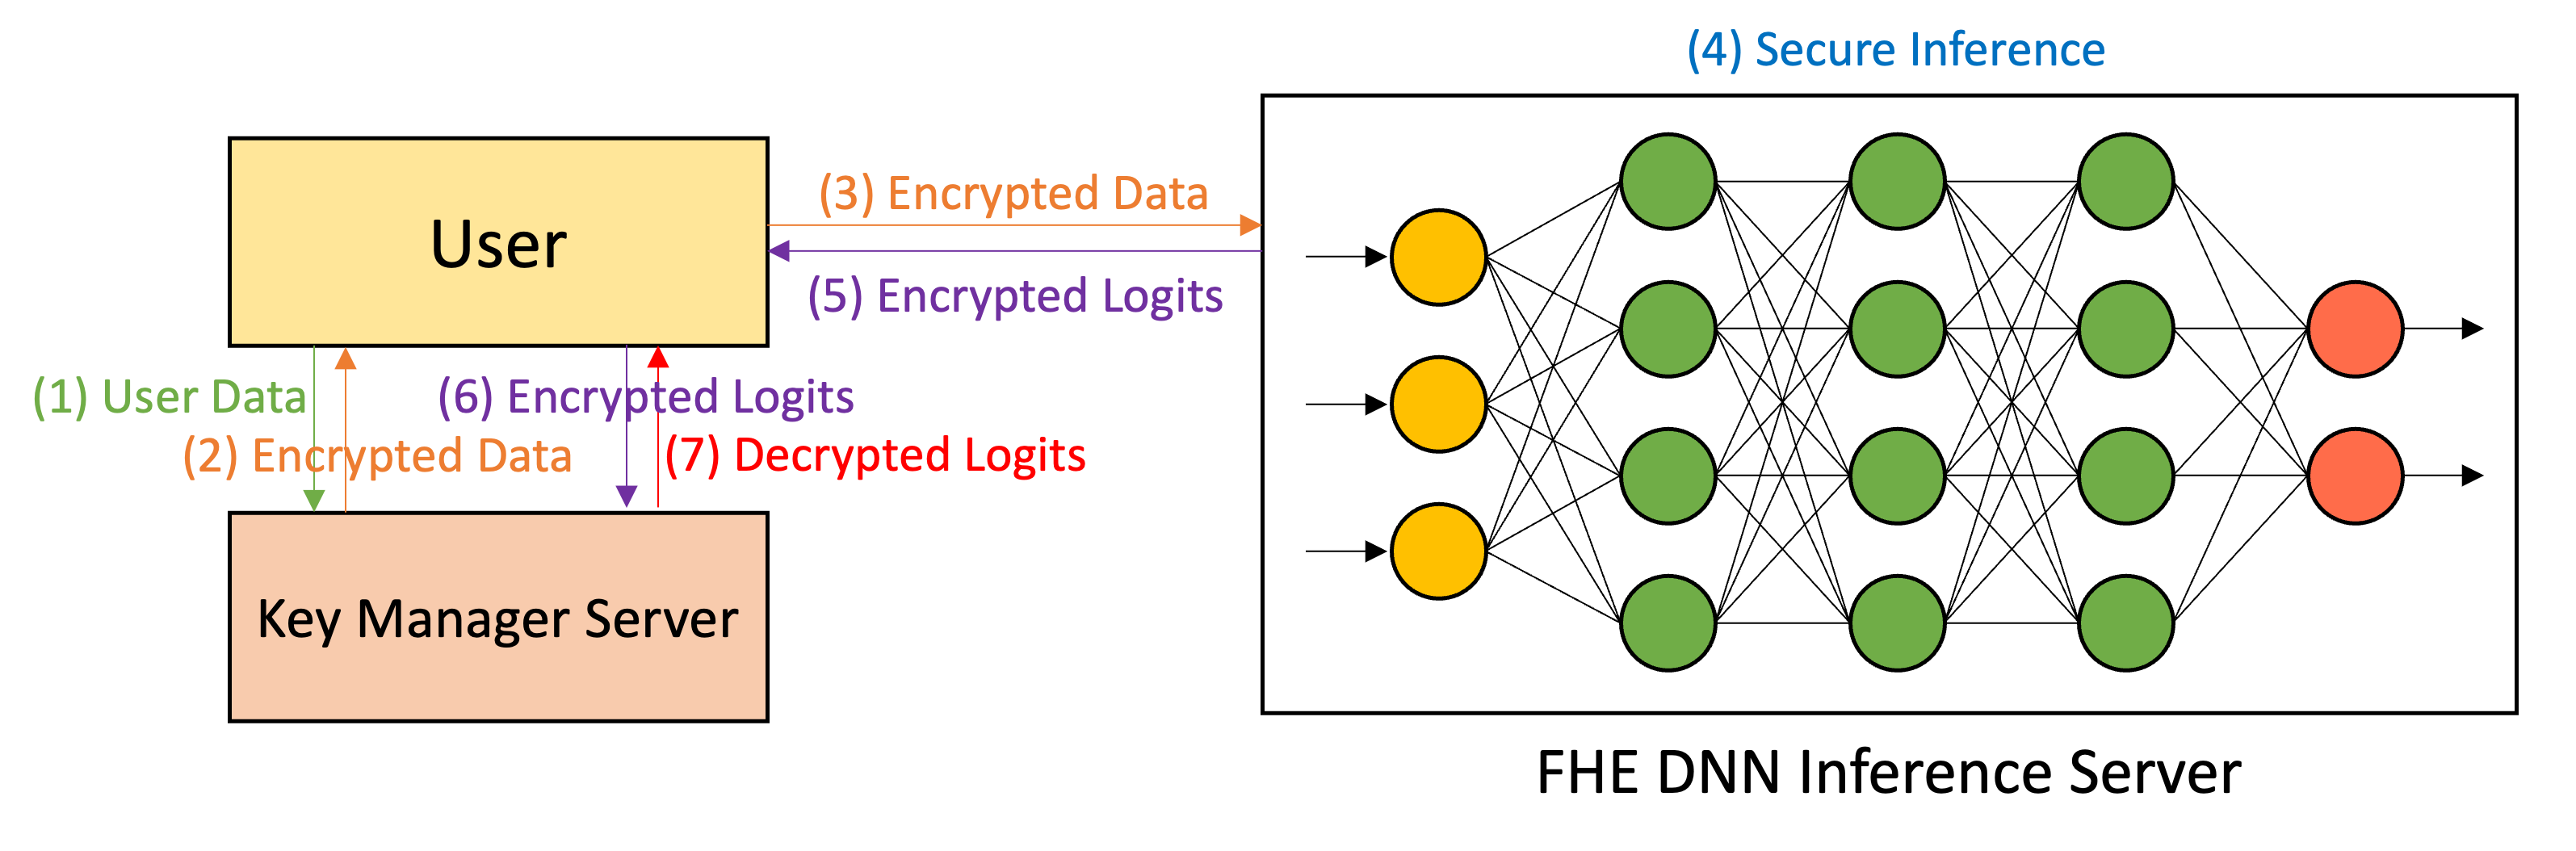
\includegraphics[width=0.7\textwidth]{resource/secure_dnn_inference.png}
        \caption{Secure DNN inference on FHE scheme}
        \label{fig:secure_dnn_inference}
    \end{figure}
\end{frame}

\begin{frame}{Secure DNN Inference on FHE}
    \begin{block}{No Conditional Instruction in HEaaN?}
        \begin{itemize}
            \item Don't know any information from the ciphertext
                  \begin{itemize}
                      \item How can one implement `$ReLU(x) = \operatorname{if}\:(x\geq 0)\:\operatorname{then}\:x\:\operatorname{else}\:0$'?
                  \end{itemize}
        \end{itemize}
    \end{block}
    \begin{alertblock}{Approximate Polynomials}
        \begin{itemize}
            \item Approximate polynomials to implement \alert{the absolute function}
                  \begin{itemize}
                      \item $|x| \approx a_0 + a_1 x + a_2 x^2 + \cdots$
                  \end{itemize}
            \item Maximum degree of the approx polynomial determines noise level drop
                  \begin{itemize}
                      \item \alert{Tradeoff between multiplicative depth v.s. accuracy}
                  \end{itemize}
        \end{itemize}
    \end{alertblock}
    \begin{gather*}
        ReLU(x) = (x + |x|) \cdot 0.5 \\
        MaxPool(x_1, x_2) = \max(x_1, x_2) = 0.5 \cdot (x_1 + x_2 + |x_1 - x_2|)
    \end{gather*}
\end{frame}

\section{Approximations}

\begin{frame}{Chebyshev's Approximation (1st Kind Expansion)}
    \begin{itemize}
        \item \alert{Known to have low average error ($mean(|f-p|)$).}
        \item Recursively generates polynomials.
              \begin{gather*}
                  T_0(x) = 1, \quad T_1(x) = x, \quad T_{n+1}(x) = 2xT_n(x) - T_{n-1}(x) \\
                  \sum_{k=1}^n T_i(x_k) T_j(x_k) = \left\{
                  \begin{array}{ll}
                      0   & \text{if $i \neq j \leq n$}  \\
                      n   & \text{if $i = j = 0$}        \\
                      n/2 & \text{if $0 < i = j \leq n$}
                  \end{array} \right.
                  \quad \text{where } x_k = -\cos(\frac{k \pi}{n})
              \end{gather*}
        \item Compute approximation coefficients similar to Fourier transformation.
              \begin{gather*}
                  f(x) \approx \sum_{i=0}^n c_i T_i(x), \quad
                  c_i = \frac{1}{d_i} \sum_{k=1}^n f(x_k) T_i(x_k), \quad
                  d_i = \left\{
                  \begin{array}{ll}
                      n   & \text{if $i = 0$}    \\
                      n/2 & \text{if $i \neq 0$}
                  \end{array}
                  \right.
              \end{gather*}
    \end{itemize}
\end{frame}

\begin{frame}{Remez's Iterative Algorithm}
    \begin{theorem}[Chebyshev's Equioscillation theorem]
        Among the approximate polynomial $p$ of $f$ s.t. $\deg(p) \leq n$,
        $||f-p||_\infty$ on a domain $[a, b]$ is minimized iff $\exists a \leq x_1 < x_2 < \cdots < x_{n+2} \leq b$
        s.t. $f(x_i) - p(x_i) = (-1)^i \cdot ||f-p||_\infty$.
    \end{theorem}
    \begin{itemize}
        \item \alert{Known to have minimal maximum error ($\max(|f-p|)$).}
        \item Iteratively fetches $x$ points and polynomial coefficients.
              \begin{itemize}
                  \item Randomly sample $n+2$ ascending data points $(x_1, x_2, \dots, x_{n+2})$ on $[-1, 1]$.
                  \item Solve a linear system of $n+2$ equations, with $n+2$ unknowns $c_0, \dots, c_n, E$:
                        \begin{gather*}
                            \left( \sum_{i=0}^n c_i x_k^i \right) + (-1)^k E = f(x_k)
                        \end{gather*}
                  \item Update $(x_1, x_2, \dots, x_{n+2})$ to have local maximums on $||f(x) - p(x)||$, and repeat from the 2nd step.
              \end{itemize}
    \end{itemize}
\end{frame}

\begin{frame}{Approximations of Absolute Function}
    \begin{figure}[!h]
        \centering
        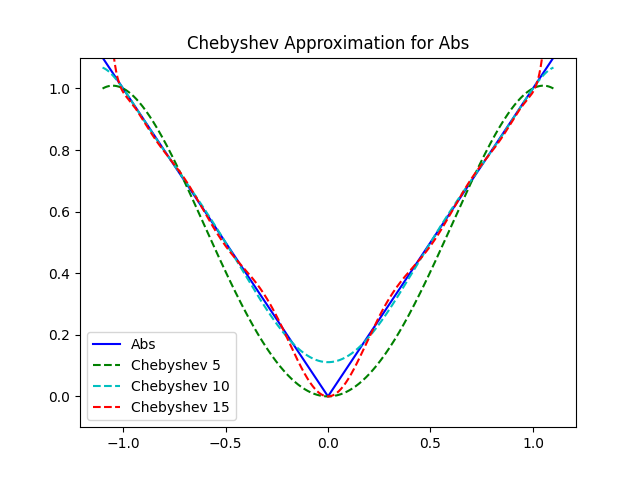
\includegraphics[width=0.45\textwidth]{resource/chebyshev.png}
        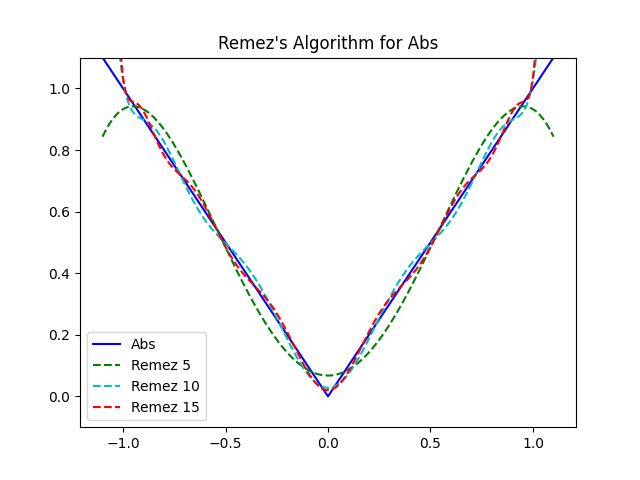
\includegraphics[width=0.45\textwidth]{resource/remez.png}
        \caption{Chebyshev's (L), Remez's approximation of absolute function $y = |x|$ (R)}
        \label{fig:approximates_absolute}
    \end{figure}
    \begin{itemize}
        \item Chebyshev has low average error, Remez's has low maximum error.
        \item Higher degree polynomials are more accurate.
    \end{itemize}
\end{frame}

\begin{frame}{Importance of Input Range Issue}
    \textit{Recall that} $ReLU(x) = (x + |x|) \cdot 0.5$
    \begin{figure}[!h]
        \centering
        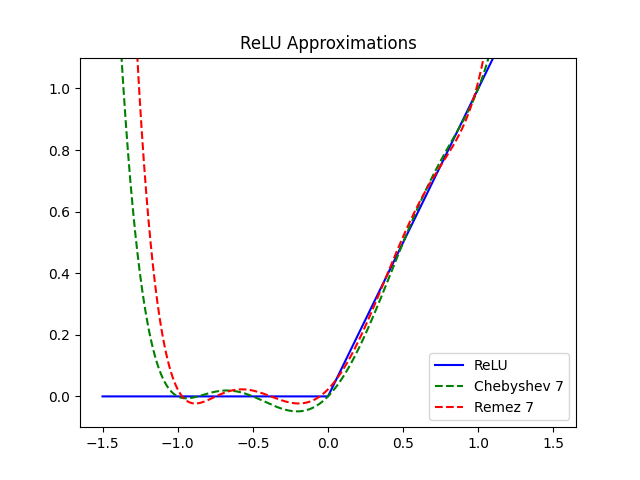
\includegraphics[width=0.6\textwidth]{resource/relu.png}
        \caption{Approximations of ReLU. The function is \alert{highly inaccurate out of $[-1, 1]$ input range.}}
        \label{fig:approximates_relu}
    \end{figure}
\end{frame}

\section{Experiments}

\begin{frame}{Experiment Environments}
    \begin{block}{Target Datasets and Networks}
        \begin{itemize}
            \item MNIST handwritten digit classification dataset.
            \item Simple convolutional classifier neural network.
                  \begin{itemize}
                      \item \texttt{Conv2d}, \texttt{Linear}, \texttt{ReLU} and \texttt{MaxPool2d} in pytorch.
                  \end{itemize}
            \item Implemented with PyTorch for secure inference simulation.
                  \begin{itemize}
                      \item \alert{Use approximation polynomials when inferencing.}
                      \item Not necessary for training phase.
                  \end{itemize}
        \end{itemize}
    \end{block}
    \begin{figure}[!h]
        \centering
        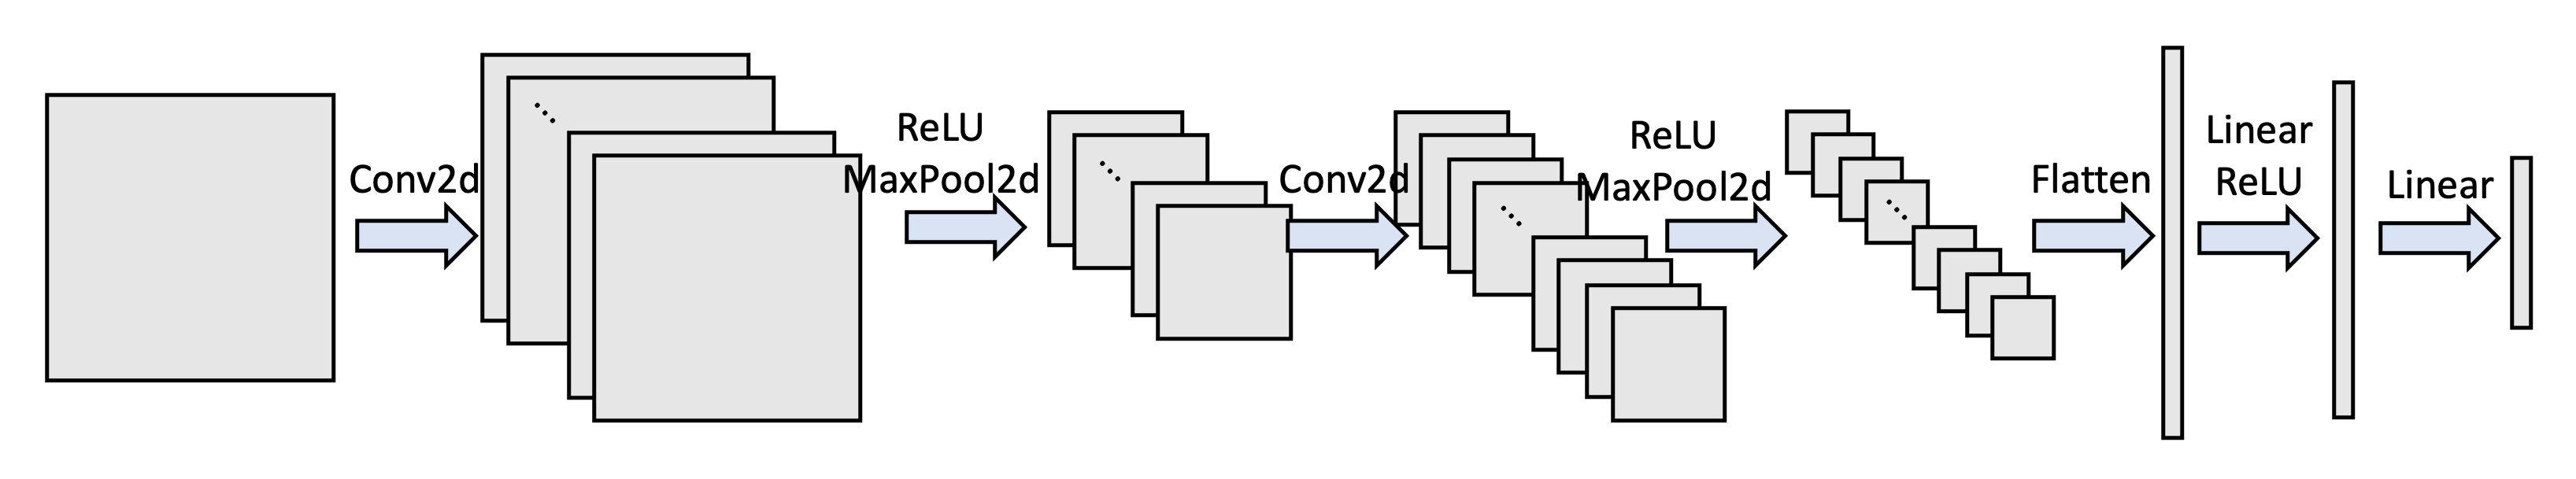
\includegraphics[width=.95\textwidth]{resource/network.png}
        \caption{Classifier Network}
        \label{fig:network}
    \end{figure}
\end{frame}

\begin{frame}{Optimization \& Fine-Tuning}
    \begin{block}{ML Components and Losses}
        \begin{itemize}
            \item \alert{Activation decay;} to reduce input norms of approx. polynomials.
                  \begin{gather*}
                      Loss(\theta, \vec x) = Loss_{orig}(\theta, \vec x) + \lambda_{act} \cdot
                      \left( \frac{1}{N} \cdot \sum_{\vec u \in \text{inputs of approx.}} ||\vec u||_p \right)
                  \end{gather*}
            \item Negative slope ($u \in [0, 1)$) on ReLU (LeakyReLU)
                  \begin{gather*}
                      LeakyReLU(x) = \left\{ \begin{array}{ll}
                          x  & \text{if $x \geq 0$} \\
                          ux & \text{if $x < 0$}
                      \end{array} \right. = \left( x + \frac{1-u}{1+u}\cdot |x| \right) \cdot \frac{1+u}{2}
                  \end{gather*}
        \end{itemize}
    \end{block}
    \begin{block}{Fine-tuning}
        \begin{itemize}
            \item Fine-tune with approximates
            \item Gradient descent training after switching HE-incompatible components into approximates
        \end{itemize}
    \end{block}
\end{frame}

\begin{frame}{Experiment Pipelines}
    \begin{alertblock}{Common Training Pipelines}
        \begin{enumerate}
            \item Train the network w/ small activation decay ($\lambda_{act,1} = 10^{-4}$) for 20 epochs
                  \begin{itemize}
                      \item Learning rates: $0.1$(10 epochs) $\rightarrow$ $0.01$(15 epochs) $\rightarrow$ $0.001$(20 epochs)
                  \end{itemize}
            \item Train the network w/ \alert{large activation decay} ($\lambda_{act,2} = 10^{-2}$) for 10 epochs
                  \begin{itemize}
                      \item Learning rates: $10^{-3}$ $\rightarrow$ $10^{-4}$ $\rightarrow$ $10^{-5}$
                  \end{itemize}
            \item \alert{Fine-tune the network by replacing} HE-incompatible components into approximates for 10 epochs ($\lambda_{act,3} = 10^{-2}$).
                  \begin{itemize}
                      \item Learning rates: $10^{-3}$ $\rightarrow$ $10^{-4}$ $\rightarrow$ $10^{-5}$
                  \end{itemize}
        \end{enumerate}
    \end{alertblock}
    \begin{block}{Control Variables}
        \begin{itemize}
            \item Approximation methods (Chebyshev v.s. Remez) and degrees
            \item Using LeakyReLU instead of ReLU
            \item Using $L2$ or $L1$-norm as activation decay
            \item Final activation decay parameter scale ($\lambda_{act,3}$)
        \end{itemize}
    \end{block}
    Github: {\small\url{https://github.com/lego0901/fhe_secure_inference_simulation}}
\end{frame}

\section{Results}

\begin{frame}{Results - LeakyReLU on L1 Activation Decay}
    \begin{figure}[!h]
        \centering
        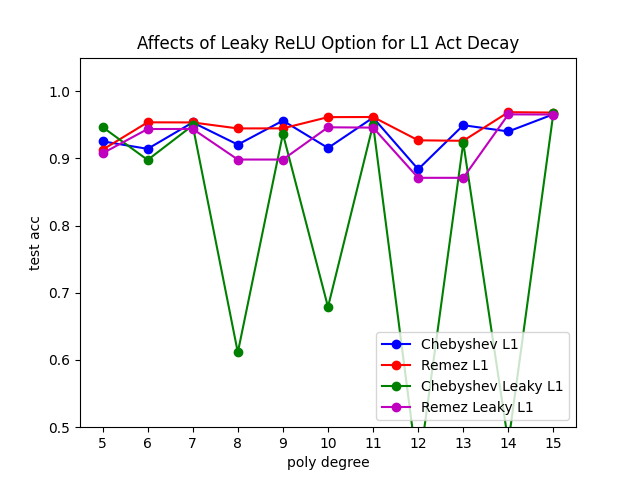
\includegraphics[width=0.75\textwidth]{resource/leaky.png}
        \caption{Affects of LeakyReLU. ReLU was more stable for $L1$ activation decay.}
        \label{fig:affects_leaky_l1}
    \end{figure}
\end{frame}

\begin{frame}{Results - LeakyReLU on L2 Activation Decay}
    \begin{figure}[!h]
        \centering
        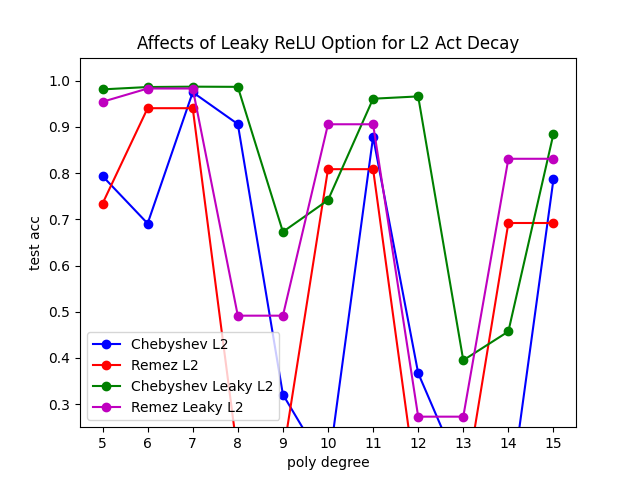
\includegraphics[width=0.75\textwidth]{resource/leaky_l2.png}
        \caption{Affects of LeakyReLU. LeakyReLU was generally better for $L2$ activation decay.}
        \label{fig:affects_leaky_l2}
    \end{figure}
\end{frame}

\begin{frame}{Results - L1 or L2 Activation Decay Norms}
    \begin{figure}[!h]
        \centering
        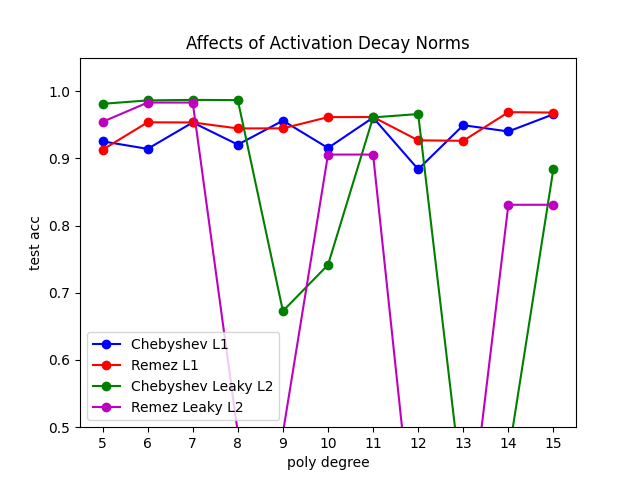
\includegraphics[width=0.75\textwidth]{resource/norm.png}
        \caption{Affects of L1 and L2 activation decay norms. L2 gave impressive performances for some cases, but L1 was more stable.}
        \label{fig:affects_norm}
    \end{figure}
\end{frame}

\begin{frame}{Results - Activation Decay Strength ($\lambda_{act,3}$)}
    \begin{figure}[!h]
        \centering
        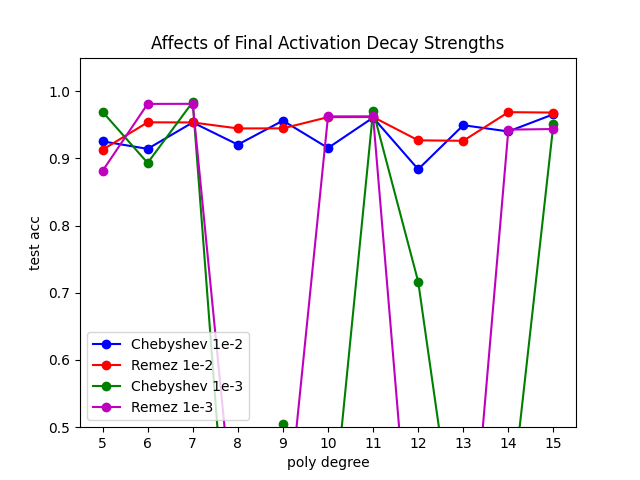
\includegraphics[width=0.75\textwidth]{resource/decay.png}
        \caption{Affects of the last activation decay term ($\lambda_{act,3}$). $10^{-3}$ gave impressive performances for some cases, but $10^{-2}$ was more stable.}
        \label{fig:affects_decay}
    \end{figure}
\end{frame}

\begin{frame}{Results - Affects of The Fine-tune Phase}
    \begin{figure}[!h]
        \centering
        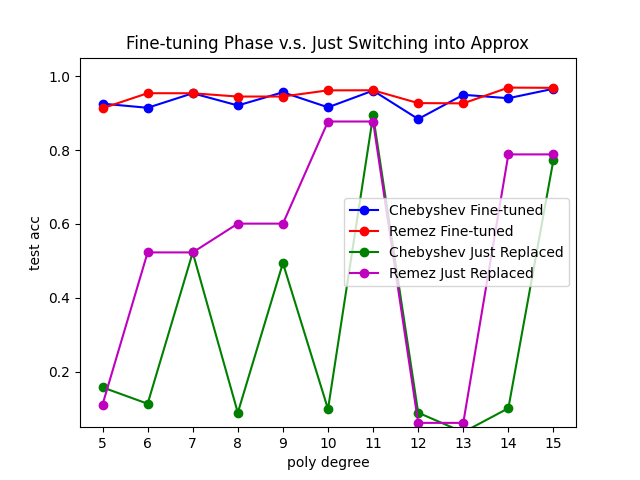
\includegraphics[width=0.75\textwidth]{resource/finetune.png}
        \caption{Affects of the fine-tuning phase. Just replacing ReLU and MaxPool2d into Approximates without fine-tuning gave poor performances.}
        \label{fig:affects_finetune}
    \end{figure}
\end{frame}

\begin{frame}{Results - Affects of The Large Activation Decay Phase}
    \begin{figure}[!h]
        \centering
        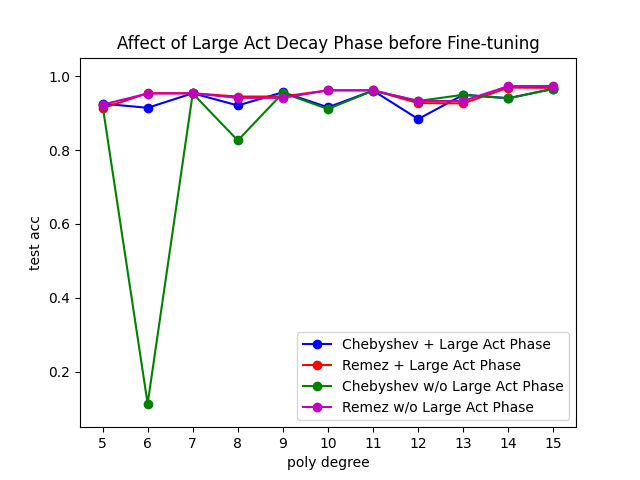
\includegraphics[width=0.75\textwidth]{resource/act.png}
        \caption{Affects of the (2nd) large activation decay phase. It provided more stable results for smaller approximation polynomial degrees.}
        \label{fig:affects_act}
    \end{figure}
\end{frame}

\begin{frame}{Results - Activation Magnitude Profiles}
    \begin{figure}[!h]
        \centering
        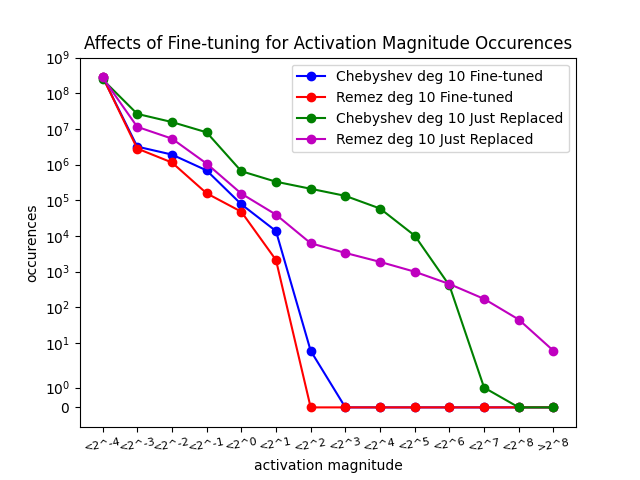
\includegraphics[width=0.75\textwidth]{resource/finetune_profile.png}
        \caption{Activation magnitude profiles. The absolute value of each activation tensor element was investigated. Fine-tuning phase reduced the activation magnitudes in genernal.}
        \label{fig:affects_finetune_profile}
    \end{figure}
\end{frame}

\begin{frame}{Results - Top Accuracies Configs}
    \begin{table}[h]
        \center
        \begin{tabular}{|c|c|c|c|} \hline
            Approximates        & Act Decay                             & ReLU Layer        & Accuracies    \\ \hline
            \alert{Chebyshev 7} & \alert{L2, $\lambda_{act,3}=10^{-2}$} & \alert{LeakyReLU} & \alert{98.71} \\
            Chebyshev 8         & L2, $\lambda_{act,3}=10^{-2}$         & LeakyReLU         & 98.67         \\
            Chebyshev 6         & L2, $\lambda_{act,3}=10^{-2}$         & LeakyReLU         & 98.63         \\
            \alert{Chebyshev 7} & \alert{L1, $\lambda_{act,3}=10^{-3}$} & \alert{ReLU}      & \alert{98.39} \\
            \alert{Remez 7}     & \alert{L2, $\lambda_{act,3}=10^{-2}$} & \alert{LeakyReLU} & \alert{98.31} \\
            Remez 6             & L2, $\lambda_{act,3}=10^{-2}$         & LeakyReLU         & 98.31         \\
            Remez 10            & L2, $\lambda_{act,3}=10^{-2}$         & LeakyReLU         & 98.21         \\
            Remez 11            & L2, $\lambda_{act,3}=10^{-2}$         & LeakyReLU         & 98.21         \\
            Chebyshev 5         & L2, $\lambda_{act,3}=10^{-2}$         & LeakyReLU         & 98.12         \\
            \alert{Remez 5}     & \alert{L1, $\lambda_{act,3}=10^{-3}$} & \alert{ReLU}      & \alert{98.12} \\
            Remez 6             & L1, $\lambda_{act,3}=10^{-3}$         & ReLU              & 98.11         \\
            \hline
        \end{tabular}
        \caption{Configurations with top accuracies}
        \label{table:top_acc}
    \end{table}
\end{frame}

\begin{frame}{Results - Activation Magnitude Profiles}
    \begin{figure}[!h]
        \centering
        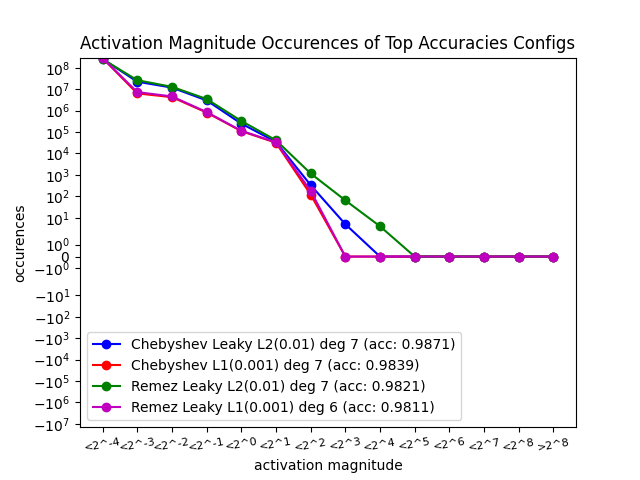
\includegraphics[width=0.75\textwidth]{resource/tops_profile.png}
        \caption{Activation magnitude profiles for remarkable configurations.}
        \label{fig:affects_top_acc_profile}
    \end{figure}
\end{frame}

\section{Conclusion}

\begin{frame}{Conclusion}
    \begin{alertblock}{Summary}
        \begin{itemize}
            \item Can switch HE-incompatible components into approximates.
            \item The accuracy drops were not critical in MNIST dataset. ($98.71\%$ in best)
            \item Fine-tuning phases were important to obtain better results.
                  \begin{itemize}
                      \item With `large activation decay' and `fine-tuning' phases.
                      \item Fine-tuning stages reduced the magnitudes of activations, to fit into valid input ranges for the approximations; $[-1, 1]$.
                  \end{itemize}
            \item \alert{Low-degree polynomials approximations were enough. (Even better!)}
                  \begin{itemize}
                      \item About 6-7 degrees polynomials produced the best performances.
                      \item Better for all computational complexities. (resources, times, mult-depths)
                  \end{itemize}
        \end{itemize}
    \end{alertblock}
    \begin{block}{Follow-up Studies}
        \begin{itemize}
            \item Not `simulating' a secure ML inference in FHE.
                  \begin{itemize}
                      \item Need to implement \texttt{Matmul}, \texttt{Conv2d}, ...
                  \end{itemize}
            \item How to optimize these technique into more complex networks.
            \item How to make a secure \alert{training} network? (not only the inference)
        \end{itemize}
    \end{block}
\end{frame}

\section{References}

\begin{frame}[t,allowframebreaks]{References}
    \nocite{*}
    \printbibliography
\end{frame}

\end{document}